%%%%%%%%%%%%%%%%%%%%%%%%%%%%%%%%%%%%%%%%%%%%%%%%%%

%% % Preamble %%%

\documentclass{beamer}

 %redefined colors for beamer 
\definecolor{beamer@nihblue}{RGB}{0,82,136} 
\definecolor{beamer@nihgrey}{RGB}{90,91,93} 
\definecolor{beamer@uiucgray}{RGB}{210,210,210} % gray for frame title background
\definecolor{beamer@uiucgray2}{RGB}{244,244,244} 

\usetheme{AnnArbor}
\setbeamercolor{frametitle}{fg=beamer@nihblue,bg=beamer@uiucgray}
\usecolortheme{wolverine} 
  

 \setbeamercolor{normal text}{fg=black} 
 \setbeamercolor{title}{fg=white,bg=beamer@nihblue} 
 \setbeamercolor{item projected}{fg=white,bg=beamer@nihgrey} 
  
 % Boxes 
 \setbeamercolor{block title}{fg=beamer@nihgrey,bg=beamer@nihblue} 
 \setbeamercolor{block body}{fg=blue,bg=beamer@nihgrey} 
 \setbeamercolor{title in head/foot}{fg=beamer@uiucgray,bg=beamer@uiucgray} % ensures the middle portion between author name colored bar (blue) and page number (colored nihgrey color bar) is the uiuc gray option
 \setbeamercolor{author in head/foot}{fg=white,bg=beamer@nihblue} 
 \setbeamercolor{institute in head/foot}{fg=white,bg=beamer@nihgrey} 
 \setbeamercolor{date in head/foot}{fg=white,bg=beamer@nihgrey} 
 \setbeamercolor{section in head/foot}{fg=white,bg=beamer@nihblue} 
 \setbeamercolor{subsection in head/foot}{fg=white,bg=beamer@nihgrey} 


%% Bullet styles and colors %%
\setbeamercolor{itemize item}{fg=beamer@nihgrey}
\setbeamercolor{itemize subitem}{fg=beamer@nihblue}
\setbeamercolor{itemize subsubitem}{fg=beamer@nihblue}
\setbeamertemplate{itemize item}{\tiny\raise1.25pt\hbox{\donotcoloroutermaths$\blacksquare$}}            % First level item
\setbeamertemplate{itemize subitem}{\tiny\raise1.25pt\hbox{\donotcoloroutermaths$\blacktriangleright$}}      % Second level item
\setbeamertemplate{itemize subsubitem}{\tiny\raise1.25pt\hbox{\donotcoloroutermaths$\blacktriangleright$}}   % Third level item


% logo for each slide to appear in bottom right hand corner (the paperwidth value controls horizontal % placement
\logo{
\includegraphics[scale=0.08]{images-logos/nih-logo.png}\hspace*{.02\paperwidth}}


% change table of contents bullet styles to circles instead of spheres (can also use `square` as well) % change subsections to numbered list and make the font size of subsections smaller
\setbeamertemplate{section in toc}[circle]
\setbeamertemplate{subsection in toc}[subsections numbered]
\setbeamerfont{subsection in toc}{size=\scriptsize}


%% add progress bar to footline %%
\addtobeamertemplate{headline}{%
  \leavevmode%
  \hbox{%
  \begin{beamercolorbox}[wd=\paperwidth,ht=2.25ex,dp=1ex,center]{section in head/foot}%
     \insertsectionnavigationhorizontal{\paperwidth}{}{}
  \end{beamercolorbox}}%

}



%% Citations/bibtex
\usepackage[style=numeric-comp,%
            autocite=footnote,%
             backend=bibtex8,%
             firstinits=true,%. %% abbreviates first name to just letters and not full first name
             ]{biblatex}
\addbibresource{01-apha-2023-slide-deck.bib}

% redefine command for foot cite-makes it smaller
\newrobustcmd*{\footlessfullcite}{\AtNextCite{\renewbibmacro{title}{}\renewbibmacro{in:}{}\renewbibmacro{urldate}{}}\footfullcite} %remove in:', title and urldate

\AtEveryCitekey{\clearfield{pages}}  %get rid of pages from footnote citation
\AtEveryCitekey{\clearfield{issn}} %get rid of issn from footnote citation
\AtEveryCitekey{\clearfield{volume}} %get rid of volume from footnote citation
\AtEveryCitekey{\clearfield{number}} %get rid of number from footnote citation
\AtEveryCitekey{\clearfield{eprint}} %get rid of eprint from footnote citation
\AtEveryCitekey{\clearfield{url}} %get rid of url from footnote citation
\AtEveryCitekey{\clearfield{month}} %get of month from footnote citation
\AtEveryCitekey{\clearlist{language}} %get rid of language from footnote citation (note \clearlist and note clearfield
\AtEveryCitekey{\clearlist{abstract}}  %get rid of abtract from footnote citation
\setbeamerfont{footnote}{size=\tiny} %make citations tiny in the footnote


% for graph/diagram of dietary patterns
\usepackage{tikz}
\usetikzlibrary{arrows} % for arrow types in tikz



% for resizing tables
\usepackage{adjustbox}

% for multiple rows in one cell
\usepackage{pbox}

% for smaller than \tiny font
\usepackage{graphicx}

% some more colors
\usepackage{xcolor}

% for colored boxes around text
\usepackage{tcolorbox}

% multiple columns for TOC
\usepackage{multicol}

%% for github icon
\usepackage{fontawesome}
%% End of Preamble %%

%% End of Preamble %%

%%%%%%%%%%%%%%%%%%%%%%%%%%%%%%%%%%%%%%%%%%%%%%%%%%


% % title page preamble %%
\title
[]{\Large County-level Food Insecurity and COVID-19 Mortality in the United States: A Spatial
	Analysis with R-INLA}

\author[Maino Vieytes CA]{Christian Maino Vieytes, PhD, MS} % name in [ ] is what goes in  footline, the name in brackets is what goes on title page

%% Institute name and U of I workmark %%
\institute[]{

\includegraphics[scale=0.065]{images-logos/nia-logo.svg.png} } % note that the insertion  of the U of I 

%  % workmark occurs within the \institute
\date[]{ November 13, 2023} % [] removes the date from the footline

%% end title page preamble %%

%% add progress bar to footline %%
\addtobeamertemplate{headline}{%
	\leavevmode%
	\hbox{%
		\begin{beamercolorbox}[wd=\paperwidth,ht=2.25ex,dp=1ex,center]{section in head/foot}%
			\insertsectionnavigationhorizontal{\paperwidth}{}{}
	\end{beamercolorbox}}%
	
}


	% following lines ensure top color bar is consistent solid color and touches top of page
\setbeamertemplate{headline}{  
	\begin{beamercolorbox}[ht=6ex,wd=1\textwidth]{section in head/foot}
	\end{beamercolorbox} %
	% redefine headline locally for title frame
}

%% Start of Document %%
\begin{document}
	



% now begin title frame
	\begin{frame}
	\titlepage{}
\end{frame}

% define FI
\subsection{What is Food Insecurity?}
\begin{frame}
	\frametitle{Defining Food Insecurity}
	
	
	According to the United States Dept. of Agriculture (USDA) \textbf{food insecurity} is defined as: \textit{a lack of consistent access to enough food for every person in a household to live an active, healthy life.}
	
\end{frame}

\begin{frame}
	\frametitle{FI in the United States}
	\begin{itemize}
		\item 13.8 million FI households  across the U.S. (10.5\%) in 2020\footlessfullcite{coleman-jensen_household_2020}
		\begin{itemize}
			\item Low-income\footnote{Household income below 130\% of the poverty line}  households: 31.2\% prevalence in 2021\footlessfullcite{coleman-jensen_statistical_2022}
		\end{itemize}
		\item Racism and housing inequality
		\begin{itemize}
			\item Housing/redlining and supermarket redlining\footlessfullcite{shaker_redlining_2022}
		\end{itemize}       
		\item Government welfare programs mitigate FI \footlessfullcite{swann_household_2017}    \begin{itemize}
			\item The Supplemental Nutrition Assistance Program (SNAP)
			\item Women, Infants, and Children (WIC)
			\item The National School Lunch Program
		\end{itemize}
	\end{itemize}
\end{frame}



%% FI and health outcomes

\begin{frame}
	\frametitle{FI and Health Outcomes}
	
	\begin{itemize}
		\item FI is associated with deleterious health outcomes\footlessfullcite{gundersen_food_2015}$^{,}$\footlessfullcite{seligman_hunger_2010}
		\begin{itemize}
			\item Hypertension
			\item Hyperlipidemia
			\item Depression and suicidal ideation
			\item Diabetes mellitus
			\item Iron deficiency anemia
		\end{itemize}
		
		\item Posited mechanisms
		\begin{itemize}
			\item Cortisol
			\item Diet quality, inflammation
			\item Competing demands and trade-offs
		\end{itemize}
	\end{itemize}
\end{frame}

  %hypotheses and rq
\section{U.S. County FI and COVID-19 Mortality}
\subsection{Research Question and Hypothesis}

%hypotheses and rq
\begin{frame}
	
	\begin{center}
		\textbf{Research Question}: \textit{Is county-level food insecurity associated with COVID-19 mortality during the first 1.5 years of the COVID-19 pandemic?}\\
		
		\vspace{1.5cm}
		
		\textbf{Hypothesis}: We hypothesize that county-level food insecurity, given its association with other health outcomes, will adversely predict county-level COVID-19 deaths.
	\end{center}
\end{frame}

 \subsection{Methods I}
\begin{frame}
	\frametitle{Analysis Plan}
\begin{itemize}
	\item Variables
	\begin{itemize}
		\item \textit{Dependent variable}: \textbf{County-level COVID-19 count}
		\begin{itemize}
			\item \textit{Source \#1}: John Hopkins University Coronavirus Resource Center (age-standardized via \textit{indirect standardization})
			\item \textit{Source \#2}: Provisional CDC restricted access individual-level data (age-standardized via \textit{direct standardization})
			\item \textit{Time window}: 03/25/2020-12/25/2021
		\end{itemize}
		\vspace{0.2cm}
		\item \textit{Independent variable}: \textbf{County-level food insecurity prevalence (2020)} (\textit{source}: Feeding America's Map the Meal Gap)
		\vspace{0.2cm}
		\vspace{0.2cm}
	\end{itemize}
\end{itemize}
\end{frame}


\begin{frame}
	\frametitle{Covariates}
	\begin{minipage}{.52\textwidth}
		\hspace{-0.5cm}
		\centering
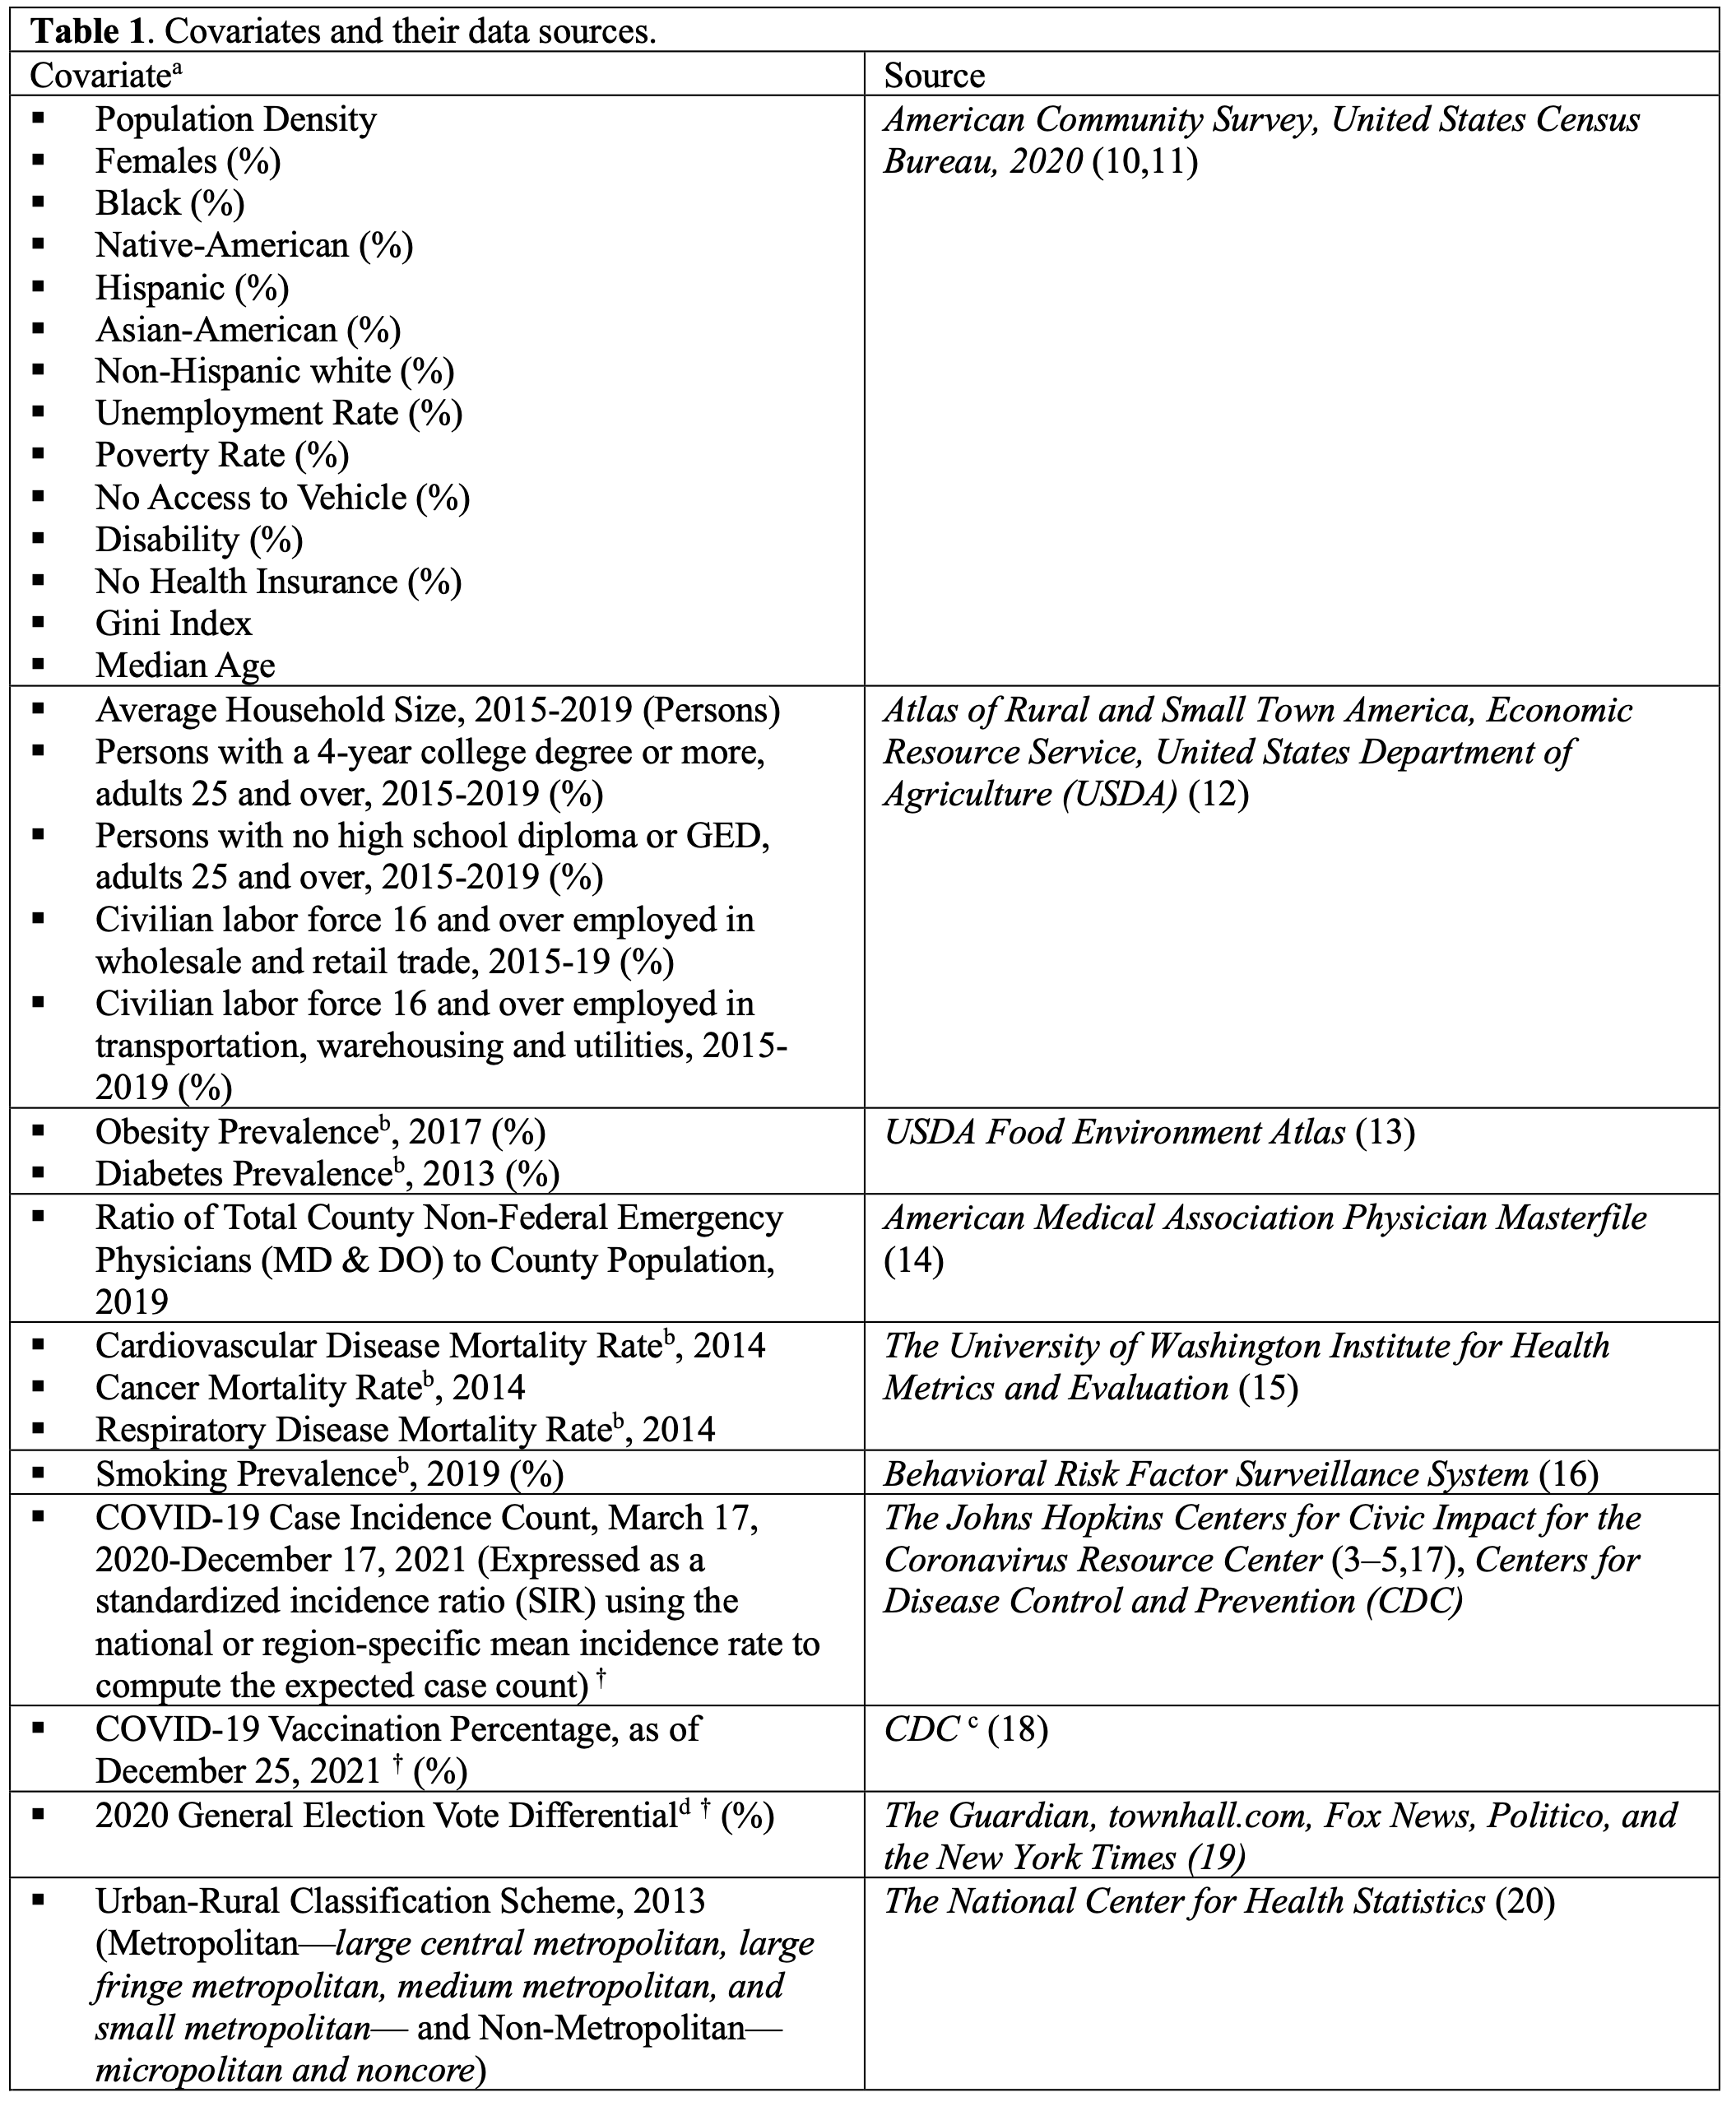
\includegraphics[scale=0.083]{images-logos/covariates-table.png}\\


	\end{minipage}% the '%' is important for putting the mini pages side by side and not stacked
	\begin{minipage}{.48\textwidth}

		\raggedleft
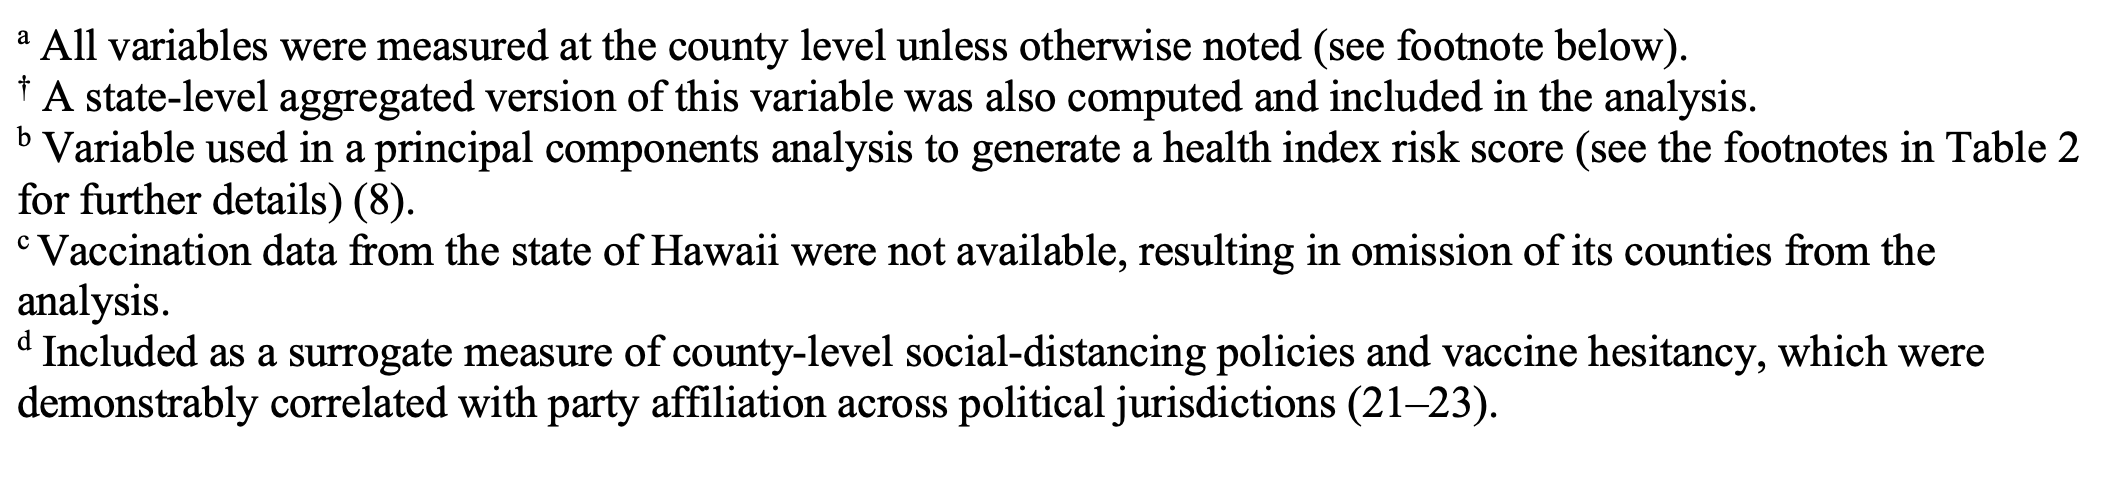
\includegraphics[scale=0.083]{images-logos/covariates-table-footer.png} 
		
		
	\end{minipage}
\end{frame}    
                \end{document}
%% End of Document %%
%%%%%%%%%%%%%%%%%%%%%%%%%%%%%%%%%%%%%%%%%%%%%%%%%%
